\hyphenation{se-para-tion}
\hyphenation{theo-re-ti-cal}
\hyphenation{handed-ness}
\hyphenation{fo-llo-wing}
\hyphenation{ac-cor-ding}

%______________________ Theory ______________________
\chapter{Theory}
\label{ch:theory}

In the previous chapter we introduced the SM and discussed particles and interactions that the SM as a theory describes. In this chapter we will discuss first the general mathematical formalism of the SM and in the second part we will focus on the double Higgs boson physics in the Beyond the Standard Model (BSM) theory.

%SM is the only accepted mathematical theory that has been extremely successful describing the interactions of elementary particles and fields. SM includes all known interactions except gravity. 

%______________________ INTRODUCCION ______________________
\section{Lagrangian formalism of the Standard Model}


The SM uses the Lagrangian mechanics as the mathematical approach to describe quantitatively the interactions of elementary particles and fields. 
The SM Lagrangian can be split into four main contributions \cite{Mozer:2016wzi}:
\begin{equation}\label{lagr_SM}
\Lagr_{SM} = \Lagr_{YM} + \Lagr_{ferm} + \Lagr_{H} + \Lagr_{Yuk} 
\end{equation}

This equation contains the following terms:

\begin{itemize}
\item gause bosons and their interactions, $\Lagr_{YM} $
\item fermions and their interactions with the gauge bosons, $\Lagr_{ferm}$
\item Higgs boson, its self-interaction, and interaction with the gauge bosons to give them mass, $\Lagr_{H}$%, which is not possible solely by the $\Lagr_{YM}$
\item fermions and their interactions with the Higgs boson, which through the Yukawa mechanism give mass to fermions, $\Lagr_{Yuk} $
\end{itemize}
 


The first term in the SM Lagrangian in full can be written as:
\beqn\label{lagr_YM}
\Lagr_{YM} = 	-\frac{1}{4}W^i_{\mu\nu}(x)W_i^{\mu\nu}(x) -\frac{1}{4}B_{\mu\nu}(x)B^{\mu\nu}(x) -\frac{1}{4}G^a_{\mu\nu}(x)G_a^{\mu\nu}(x)
\eeqn

where

\begin{align}
B_{\mu\nu}(x)   \equiv & \partial_\mu B_\nu -  \partial_\nu B_\mu \label{B_tensor} \\ 
W^i_{\mu\nu}(x) \equiv & \partial_\mu W^i_\nu(x) - \partial_\nu W^i_\mu(x) - g\varepsilon^{ijk}W^j_\mu W^k_\nu \label{W_tensor}\\
G^a_{\mu\nu}(x) \equiv & \partial_\mu G^a_\nu(x) - \partial_\nu G^a_\mu(x) - g_s f^{abc}G^b_\mu G^c_\nu \label{G_tensor}
\end{align}

\noindent with indexes $i,j,k = 1,2,3$ and $a,b,c = 1, ..., 8$. According to the Noether's theorem, each symmetry is intrinsically connected to the conservation law \cite{Sardanashvily:2143630}. The fields in the $\Lagr_{YM} $ are connected to their corresponding underlying symmetries in the following way: $B_{\mu\nu}$ corresponds to $U(1)$ symmetry of the weak hypercharge $Y_k$, $W^i_{\mu\nu}$ corresponds to $SU(2)_I$ symmetry of the weak isospin $I^i_{w}$, and $G^a_{\mu\nu}$ corresponds to $SU(3)_c$ symmetry of the QCD color charge. The "B" field is a kinematic term, "W" and "G" terms describe interactions among the bosons, $g$ and $\varepsilon$ are $SU(2)$ coupling and structure constants, $g_s$ and $f$ are coupling and structure constants for $SU(3)$.

The second term in the SM Lagrangian shows how fermions interact with the gauge bosons. Notice, that the mass terms are still absent:
\beqn\label{lagr_ferm}
\Lagr_{ferm}= i \bar{\Psi}_L \slashed{D} \Psi_L  + i \bar{\psi}_{l_{R}}  \slashed{D} \psi_{l_{R}} +
i \bar{\Psi}_Q \slashed{D} \Psi_Q  + i \bar{\psi}_{u_{R}}  \slashed{D} \psi_{u_{R}} +
 i \bar{\psi}_{d_{R}}  \slashed{D} \psi_{d_{R}}
\eeqn

Above $\Psi$ represents a doublet of a charged lepton and a corresponding neutral lepton within the same lepton family of $SU(2)_L$, the letter Q is reserved for a family of quarks, and $\psi_R$ describes a right-handed leptonic singlet.  Gauge boson interactions are present due to the derivative term:
\begin{align}\label{cov_der2}
D_\mu = \partial_\mu + ig I_w^i W_\mu^i+ ig' Y_w B_\mu + ig_s T_c^a G_\mu^a
\end{align}

\noindent Physical fields in this notation are represented by a linear combination of W and B fields:
\begin{align}\label{neutral_fields}
A_\mu = &  B_\mu \cos\theta_W + W^3_\mu \sin\theta_W \\ 
Z_\mu = & -B_\mu \sin\theta_W + W^3_\mu \cos\theta_W \nonumber 
\end{align}
\noindent where $\theta_W$ is known as the \ti{Weinberg angle} \cite{Weinberg:799984}.

With the first two terms of the SM Lagrangian one obtains a valid theory of fermions and bosons, however, these particles are massless in this theory \cite{Wolf:2015kua}, which evidently contradicts the reality. To solve this issue and to ensure that weak bosons are massive, one has to introduce a Higgs field. Higgs mechanism enters the SM Lagrangian through the corresponding Higgs Lagrangian term given by 
\beqn\label{lagr_higgs}
\Lagr_H=(D_\mu\Phi)^\dagger(D^\mu\Phi) - V(\Phi) , \qquad V(\Phi)= - \mu^2(\Phi^\dagger\Phi) + \frac{\lambda}{4}(\Phi^\dagger\Phi)^2
\eeqn

\noindent where

\beqn\label{vev}
\Phi = \binom{\phi^+}{\phi^0 = (v+H + i\chi)/ \sqrt{2}} \quad \text{with} \quad v = 2 \sqrt{\frac{\mu^2}{\lambda}}
\eeqn

\noindent here $\mu$ and $\lambda$ are parameters of the Higgs potential. The value of the Higgs field vacuum expectation value ($vev$) $v$, after the SSB, can be expressed in terms of $\mu$ and $\lambda$. See Fig. \ref{hp2d} for an illustration of the Higgs potential before and after the SSB.

The Higgs boson mass is proportional to the $\mu$ parameter. In 2012, with precise single Higgs boson mass measurements from both ATLAS and CMS experiments, the value of $\mu$ was determined. Since that time many analyses at CERN have been targeting the measurement of the $\lambda$ parameter, because it is related to the shape of Higgs potential. The simplest interaction that is probing the Higgs potential directly is the one where the Higgs boson self-coupling is present. This double Higgs (HH) process is the main topic of this thesis. 

The importance of the $\Lagr_H$ in the SM Lagrangian is crucial: after rearranging terms the bosons finally have masses given by:

\beqn
M_W = \frac{gv}{2}, \quad  M_Z = \frac{M_W}{\cos{\theta_W}}, \quad M_H = \sqrt{2\mu^2}
\eeqn



\begin{figure}[H]
\centering
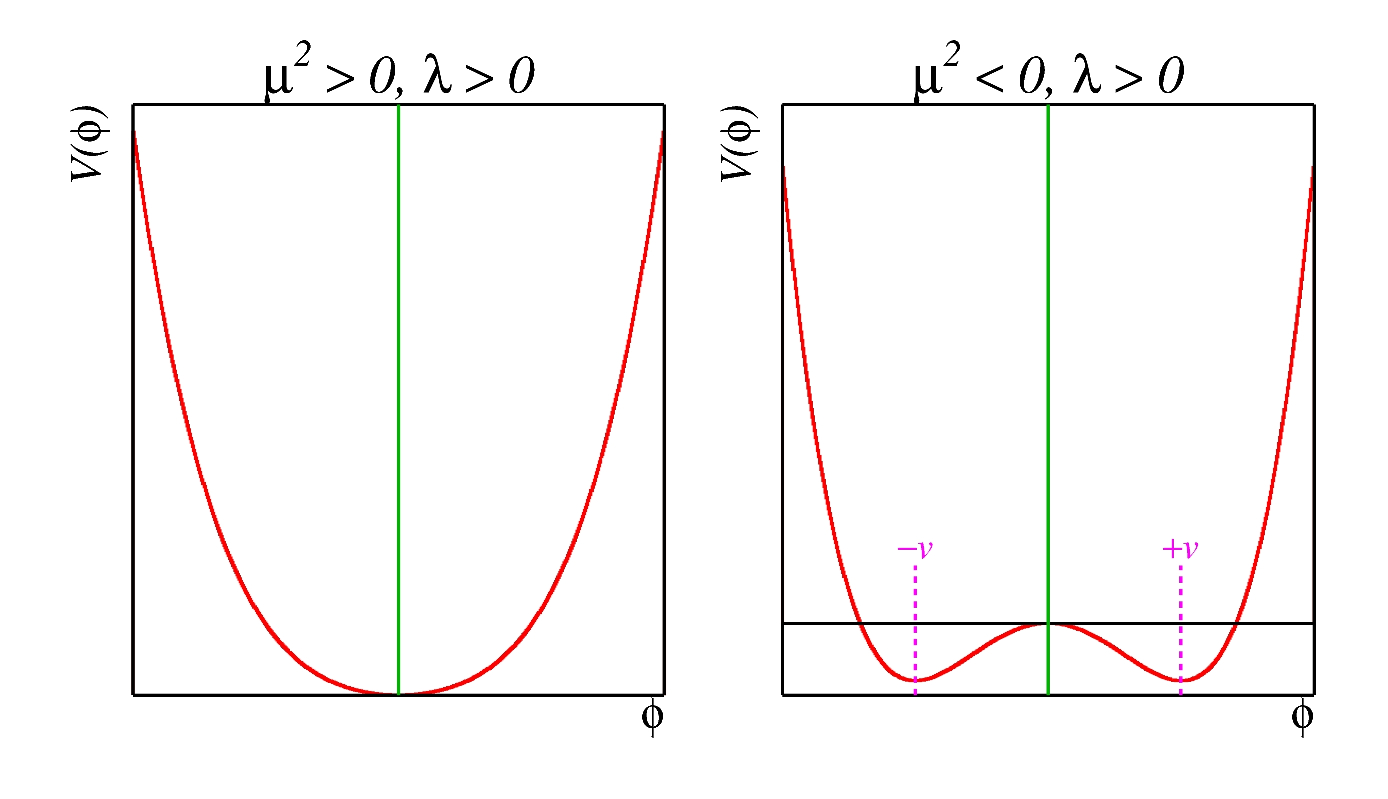
\includegraphics[width=0.6\textwidth]{hp2d}
\caption[SSB Potential form]{Shape of the Higgs potential before and after the SSB that is determined at the leading orders by $\mu$ and $\lambda$ parameters \cite{MonroyMontanez:2639240}.}
\label{hp2d}
\end{figure}



 
The final contribution to the SM Lagrangian is the Yukawa term, with Yukawa Lagrangian given by:
\beqn\label{lagr_Yuk}
\Lagr_{Yuk}=  - i \bar{\Psi}_{L}  G_l  \psi_{l_{R}} \Phi
- i \bar{\Psi}_{Q}  G_u  \psi_{u_{R}} \tilde{\Phi}
- i \bar{\Psi}_{Q}  G_d \psi_{d_{R}} \Phi + h.c.
\eeqn

\noindent where $\tilde{\Phi} = i \sigma^2 \Phi^*$. The masses of fermions enter the equations through the $3 \times 3$ matrices G, which are free parameters in the SM and have to be determined from the experiment. The mass of each fermion is proportional to the Yukawa coupling of the corresponding fermion to the Higgs boson, see Fig. \ref{coupling_ff}.


In the SM having the "Mexican hat" Higgs potential, the simplest potential characterised by $\mu$ and $\lambda$ parameters, is sufficient to obtain the SSB phenomenon. This gives mass to fermions and bosons. However, the shape of the Higgs potential may be different and direct precise determination of the $\mu$ and $\lambda$ parameters is a sensitive tool to test the limitations of the SM and may open doors to the BSM effects. All this makes HH physics one of the main goals for the future High Luminosity LHC (HL-LHC).

While mass parameter has been measured fairly accurately, $\lambda$ parameter requires even HL-LHC to run for many years to get enough statistics since HH processes are rare and are of almost three orders of magnitude lower rate than the single Higgs boson production. Technically, the amount of the HL-LHC data is not enough to reach the sensitivity of the SM for HH processes. At the same time, several BSM models predict resonant HH production to which even the current LHC data could be sensitive. In this theories, HH is produced through the decay of a heavy narrow width resonance, which is not a part of the SM. Thus, if such processes are found, this will open a new chapter in the HEP physics. In this thesis we focus on the resonant production of the HH system, which further decays to leptons and quarks. With the available CMS data, resonant HH analyses are starting approaching the needed sensitivity to rule out some BSM theories and test further the most promising ones.

\section{Double Higgs in Beyond the Standard Model}

Several BSM theories \cite{Huang:2017nnw, Dolan:2012ac, Kanemura:2016tan} predict a resonant production of the double Higgs boson events through a heavy resonance of a narrow width ($\sim O(1-10)$ GeV) \cite{Sirunyan:2018iwt}. In this dissertation data is compared with respect to predictions from the Warped Extra Dimensions theory (WED) \cite{Oliveira:2014kla}. WED theory to address the hierarchy problem adds additional fifth dimension to the 4-dimensional (4D) space-time. In the framework that Randall and Sundrum (RS) \cite{Randall:1999ee} introduced, 4D space is an EFT approximation of the higher dimensional space. Extra dimension exists between the gravity (Planch) and weak (TeV) flat 4D branes \ref{branes} and is called the "bulk". The bulk is described by the exponentially decaying metric. 



\begin{figure}[H]
\centering
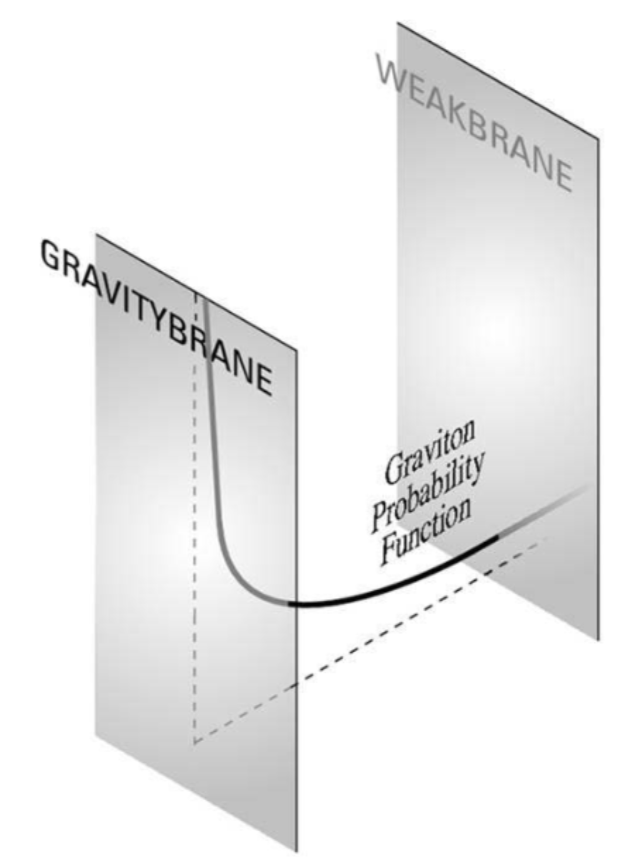
\includegraphics[width=0.4\textwidth]{branes.png}
\caption[RS branes]{5D space in the RS model \cite{Xanda}.}
\label{branes}
\end{figure}




Free parameters of the RS model are the branes separation factor $k$ and the size of the compactified dimension $r_c$. The curvature factor $k \approx \sqrt{ \frac{\Lambda}{M^2_5}  }$, where $\Lambda$ is the ultraviolet cutoff of the theory and $M_5$ is the 5D Planch mass. The radius of the extra dimension $r_c$ is proportional to the parameter $1/k$ and the logarithm of $1/vev$. The SM results with Higgs boson being closer to the TeV brane and fermions having light mass (located near the Planch brane) are reproduced with the $k \cdot r_c \approx 11$. 



Since LHC had provided us with no evidence of the SM particles interacting with the RS particles, it is postulated that the latter are confined to branes. Two new heavy particles appear in the RS theory. One is a graviton (spin 2) that is the mediator of the gravitational force. Graviton can propagate freely in the full higher-dimensional space of the 5D bulk. The weakness of the gravity is, thus, explained by the fact that the graviton is localised closer to the Planch brane. When the bulk is compactified, it may produce Kaluza-Klein (KK) \cite{Uzawa:1999pg} excitations of the gravitational field with the zero-th KK mode (graviton) localised at the TeV scale. The other RS particle is a radion (spin 0). Its existence is required to stabilise the size of the extra dimension. 


In this thesis, the RS parameters $k$ and $\bar{M}_{Pl}$ satisfy the constraint $0.01 \leq k / \bar{M}_{Pl} \leq 1$, since values outside of this range overcomplicate the model \cite{Davoudiasl:1999jd}. The parameter $k$ is of the order of the Planck scale and $\bar{M}_{Pl} = \sqrt{\frac{M^3_5}{k} \cdot (1 - e^{-2\pi k r_c} ) }$ is a reduced 4D $M_{Pl}$. Considered in this measurement graviton and radion are RS KK graviton and RS radion particles that emerge in RS scenario with a KK state mass of the order of TeV. 

Let us denote a part of the KK 5D wave function, often called a profile, as $f^{(n)}_X(\phi)$, where n is referred to the n$^{th}$ KK mode, then the graviton 4D profile wave-function can be expressed as $h^{(n)}_{\mu\nu}(x_\mu)(f^{(n)}_X(\phi))$ and the zero-th mode of this function would correspond to the graviton with the effective mass of the order of TeV. The profiles for all the matter fields are described by a combination of Bessel and exponential functions. The Lagrangian describing the interaction of the graviton with the SM fields is given then by 

\beqn\label{lagr_graviton}
\Lagr_{graviton}=  - \frac{x_1\tilde{k}}{m_G} h^{\mu\nu(1)} \times d_i T^{(i)}_{\mu\nu},  
\eeqn
where $x_1$ = 3.83 is the first zero of the Bessel function for a given profile, $\tilde{k}  = k / \bar{M}_{Pl}$, $h^{\mu\nu}$ is a symmetric tensor, $m_G$ is the effective mass of the graviton of the order of TeV, $d_i$ is an integral of the profiles of the SM fields and KK graviton, and  $T^{(i)}_{\mu\nu}$ is a 4D canonical energy-momentum tensor \cite{Forger:2003ut} for any SM field $i$. A free parameter $\tilde{k}$ varies from 0.01 to 1 when $M_{graviton}$ is varied from 100 to 1500 GeV. 

For radion the Lagrandian is given by:
\beqn\label{lagr_radion}
\Lagr_{radion}=  - \frac{r}{\Lambda_R} \times a_i T^{\mu (i)}_{\mu},  
\eeqn
where $r$ is a 5D radion field, $\Lambda_R$ is the scale parameter proportional to $k \cdot \sqrt{ ( \frac{M_5}{k} )^3}$, and $a_i$ is the coupling of the radion to the SM field $i$. RS authors assume that the profiles of the graviton and radion are localised at the TeV scale for the coupling of a radion and a graviton to the massive SM fields to be of the order of 1. 




In the SM the HH system is produced predominantly via two diagrams shown on Fig.\ref{SM_HH}: the "box" and the "triangular" diagrams. They interfere destructively and the total cross section is thus lowered (Fig. \ref{hh_comparison} on the right). The box diagram dominates the double Higgs boson production and peaks near 400 GeV. An extensive study has been performed by theorist and more details can be found at \cite{Chen:2014xra}. In this measurement, though, the gravitons and radions in the search are expected to be produced by three BSM "contact interaction" Feynman diagrams allowed by the WED scenario. These processes are given on Fig. \ref{BSM_HH}.  A graviton and a radion subsequent decays to HH system are thoroughly studied and the experimental results are compared to the theoretical predictions calculated for the WED model with the parameters $\tilde{k}=0.1$ and $\Lambda_R = 3 $ TeV.  




\begin{figure}[H]
  \centering
    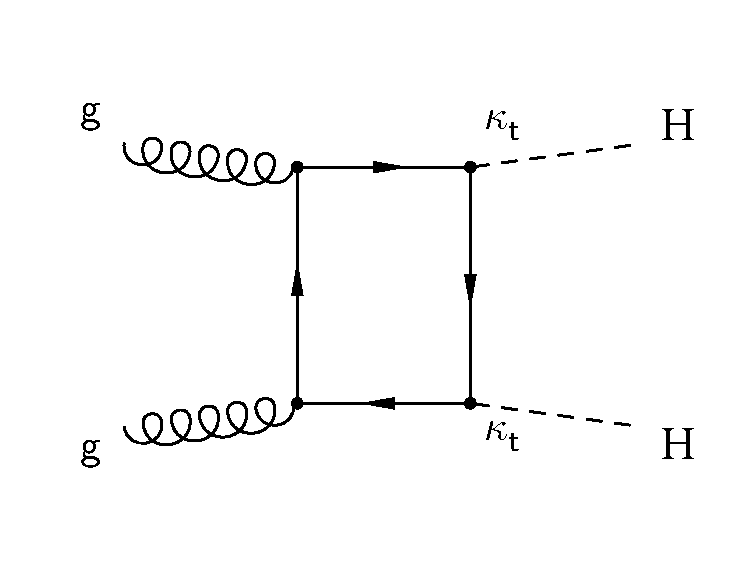
\includegraphics[width=0.49\textwidth]{hh_nonresonant_eft_02}
     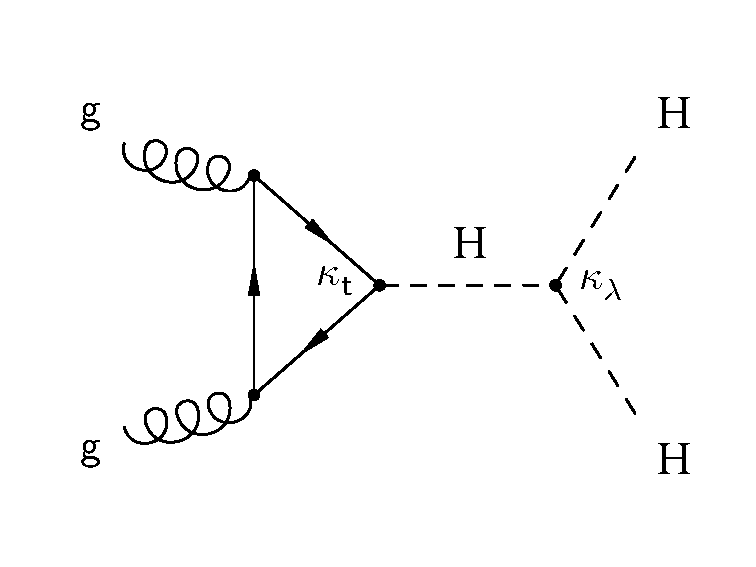
\includegraphics[width=0.49\textwidth]{hh_nonresonant_eft_01}
    \caption{SM double Higgs boson production.}
    \label{SM_HH}
\end{figure}


\begin{figure}[H]
  \centering
    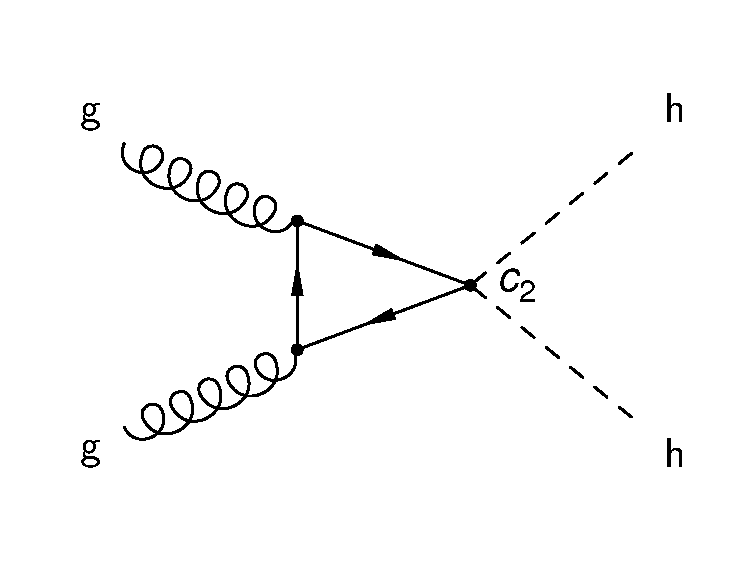
\includegraphics[width=0.49\textwidth]{hh_nonresonant_eft_03}
    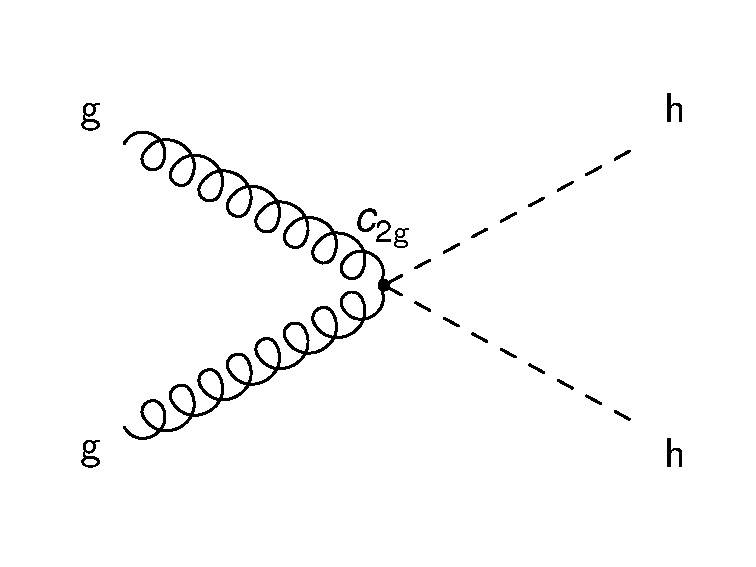
\includegraphics[width=0.49\textwidth]{hh_nonresonant_eft_04}\\
     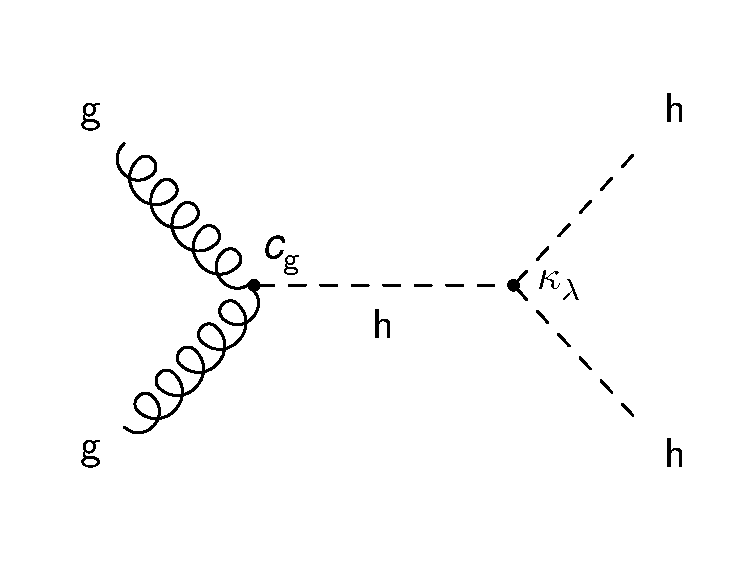
\includegraphics[width=0.49\textwidth]{hh_nonresonant_eft_05}
    \caption{BSM double Higgs boson production.}
    \label{BSM_HH}
\end{figure}



The kinematic distribution of the double Higgs mass remains to a high degree unchanged between 13-14 and 100 TeV (see Fig. \ref{hh_comparison} on the left), therefore, we can compare 100 TeV results produced by theorist to those analysed in this thesis that use the date delivered by the current 13 TeV LHC machine. Fig. \ref{hh_comparison} refers to the box and the triangular diagrams as "box" and "tri", and to the non-linear interaction as "nl"  \cite{Contino:2012xk}. 



 
 

\begin{figure}[H]
  \centering 
    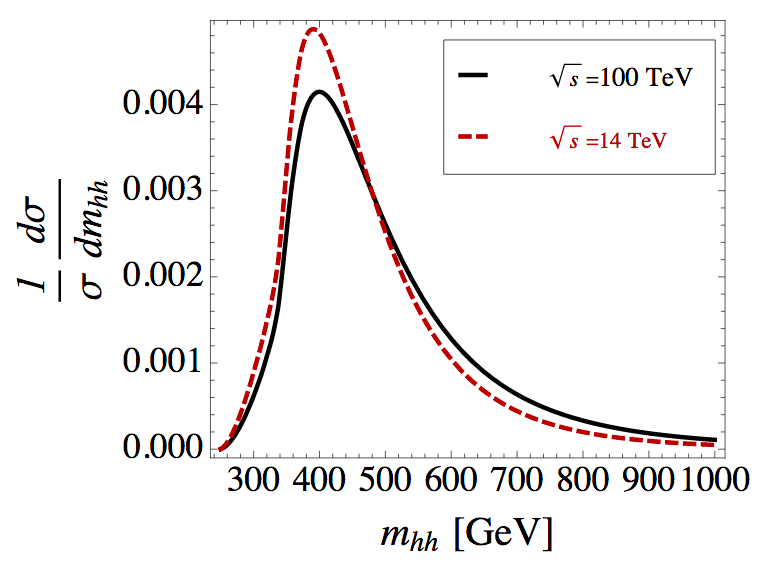
\includegraphics[width=0.49\textwidth]{hh_14_100_comparison}
    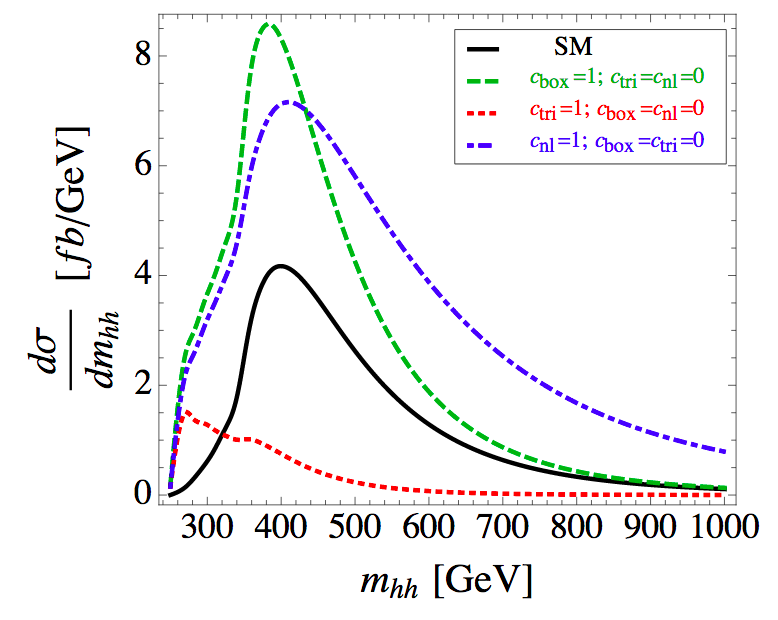
\includegraphics[width=0.49\textwidth]{hh_sm_comparison}
    \caption[Double Higgs mass distribution and the total cross-section]{Left: comparison of the double Higgs boson mass distribution at the LO at 14 and 100 TeV center-of-mass energy. Right: the total HH cross section and the individual contributions \cite{Contino:2012xk}.}
    \label{hh_comparison}
\end{figure}


From the physics point of view it is also interesting to measure BSM contact interaction couplings. The future non-resonant version of this data analysis will target such a measurement. In this case, $c_2$, the coupling of two heavy quarks with two Higgs bosons, $c_{2g}$, the coupling of two gluons with two Higgs bosons, and $c_g$, the direct coupling of the gluons to the Higgs boson will be studied (see Fig. \ref{BSM_HH}). 



This thesis addresses separately resonant graviton and radion decays into two SM Higgs bosons with the subsequent decays of one Higgs boson to a pair of b quarks, and the other Higgs boson to W or Z boson pairs. W bosons are allowed to decay only leptonically. For Z boson decays, the signature is characterised by the on-shell Z boson decaying into a pair of charged leptons and the off-shell Z boson decaying to neutrinos (see Fig. \ref{HH_signature}). The final state that this thesis focuses on consists of two b quarks, two charged leptons, and two neutrinos. This signature has a branching fraction of approximately $2.8 \%$. 

\begin{figure}[H]
  \centering
    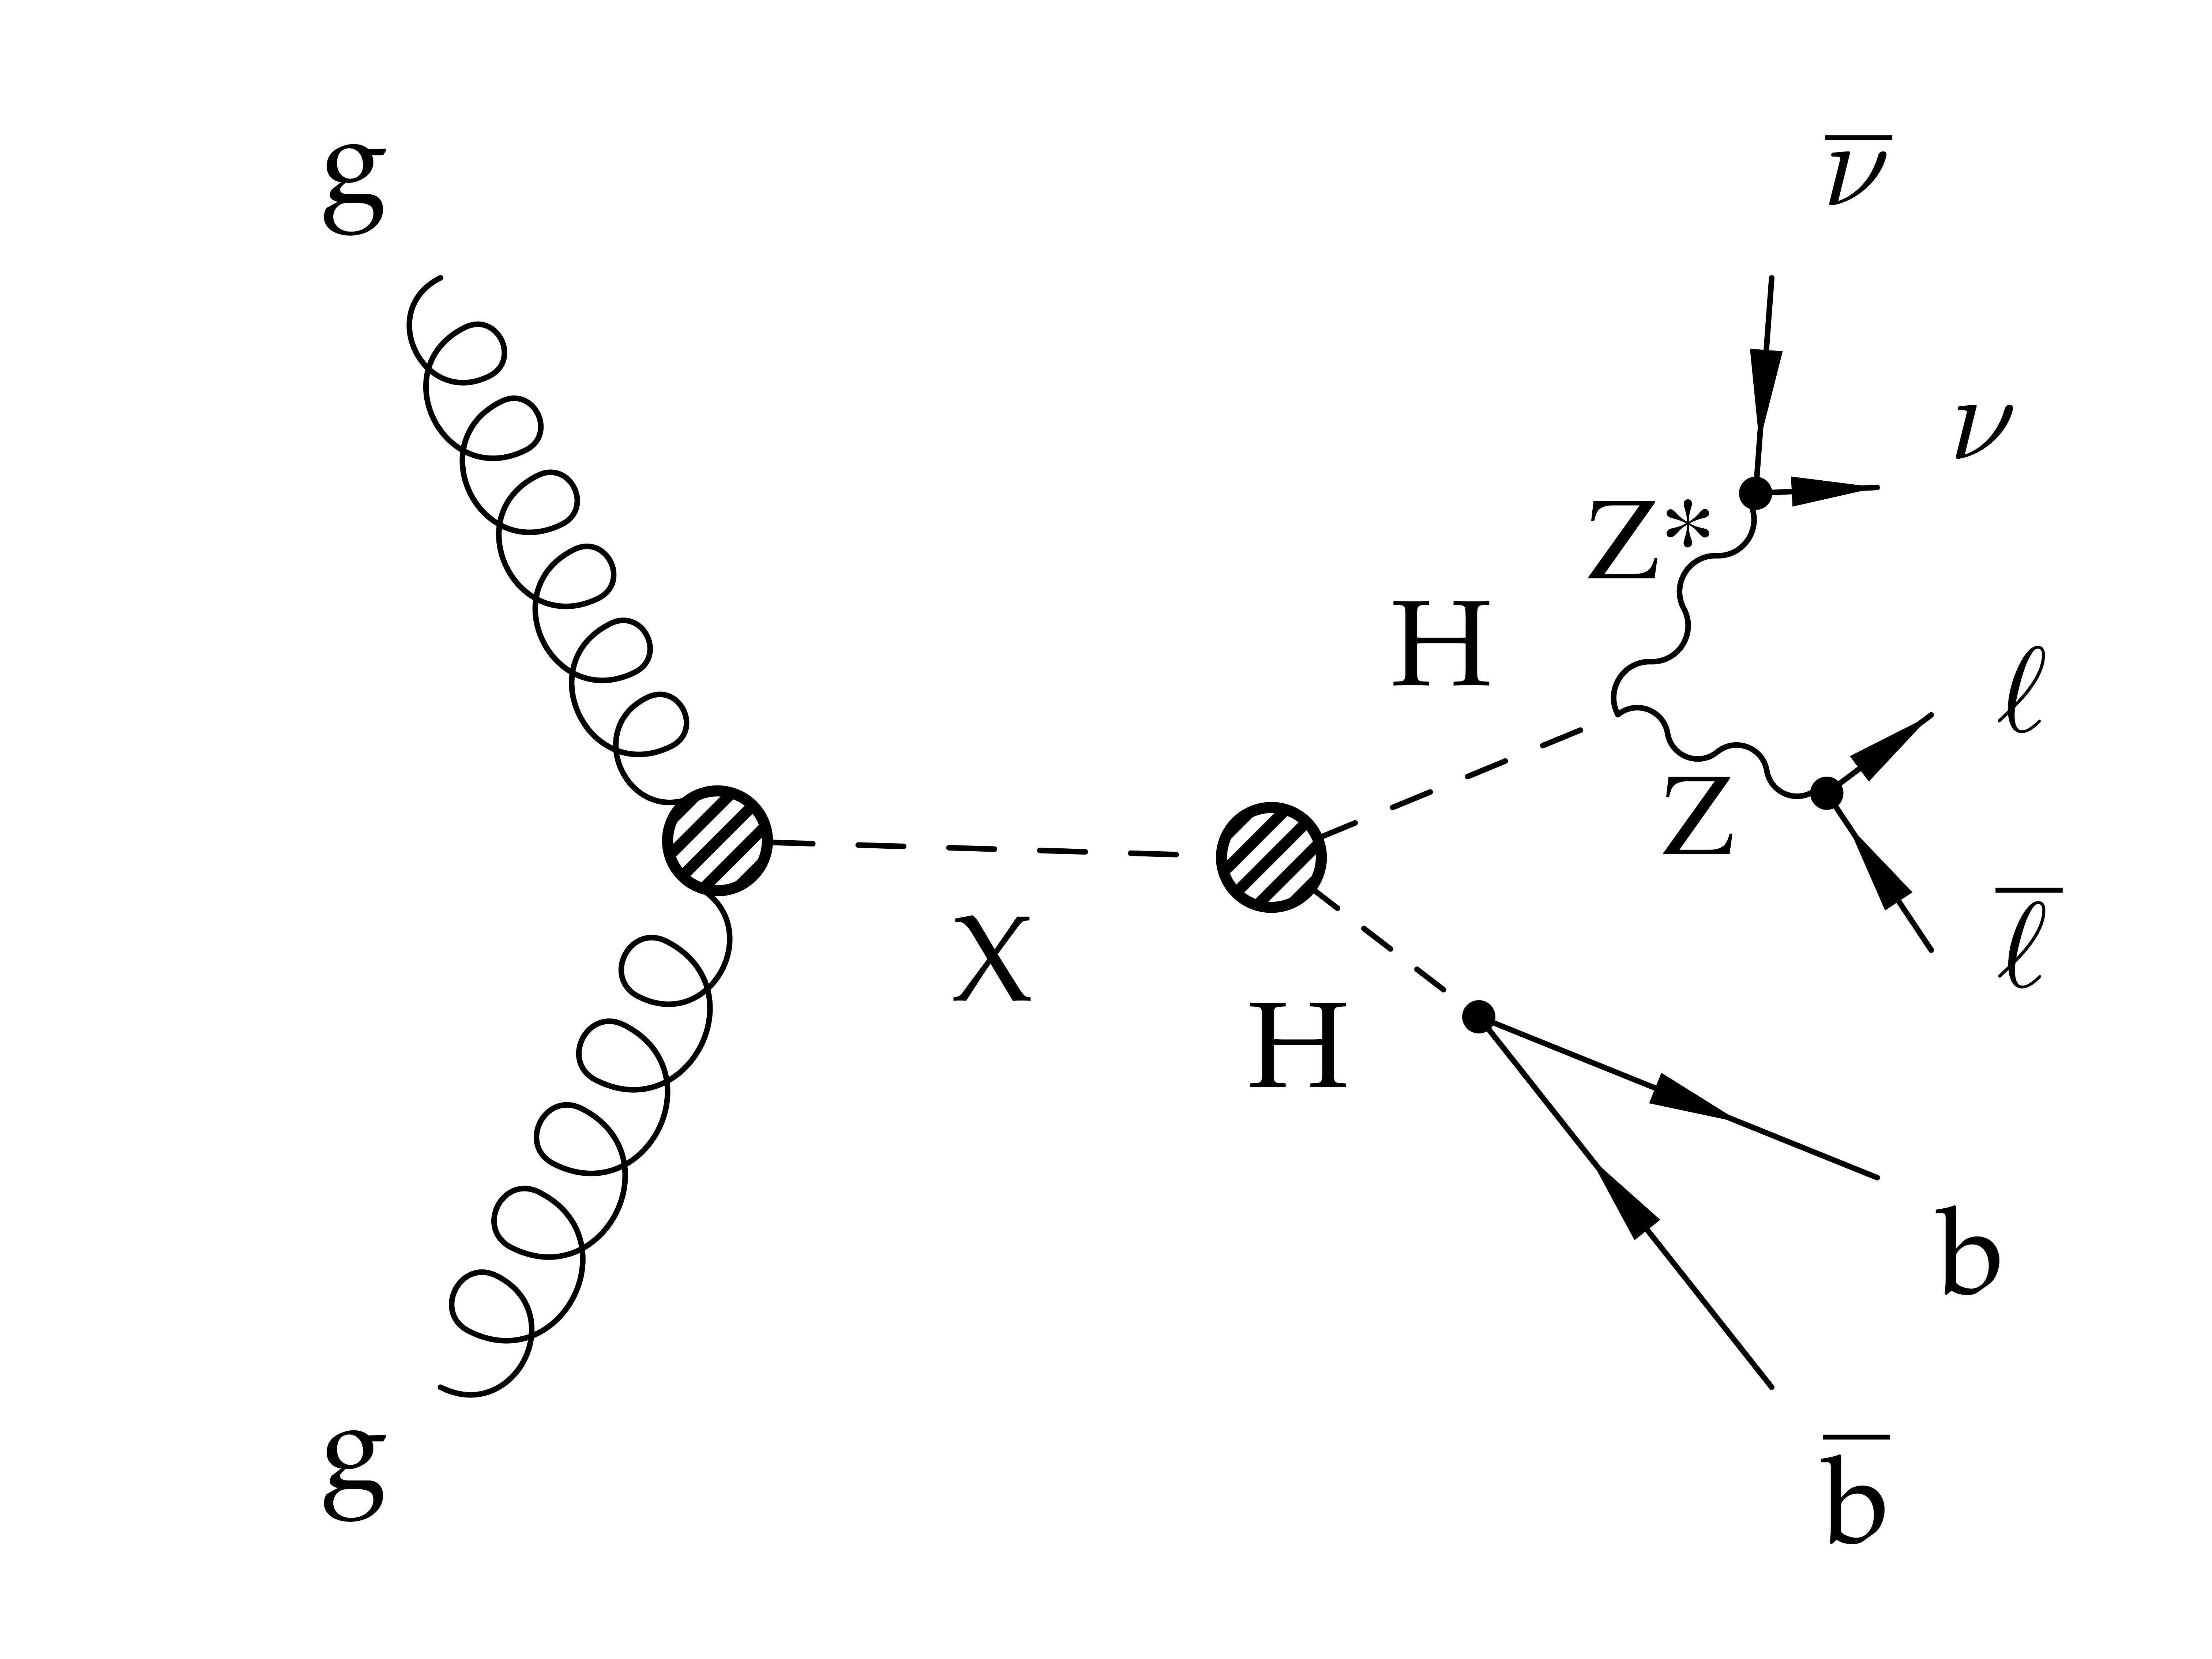
\includegraphics[width=0.50\textwidth]{HH_signature.png}
    \caption{Double Higgs decay in the 2 b, 2 lepton, and 2 neutrino final state. }
    \label{HH_signature}
\end{figure}

To finish this chapter, it is instructive to show all the decay channels of the double Higgs system to the SM particles, which is summarised in the Fig. \ref{BR}. 

\begin{figure}[H]
  \centering
    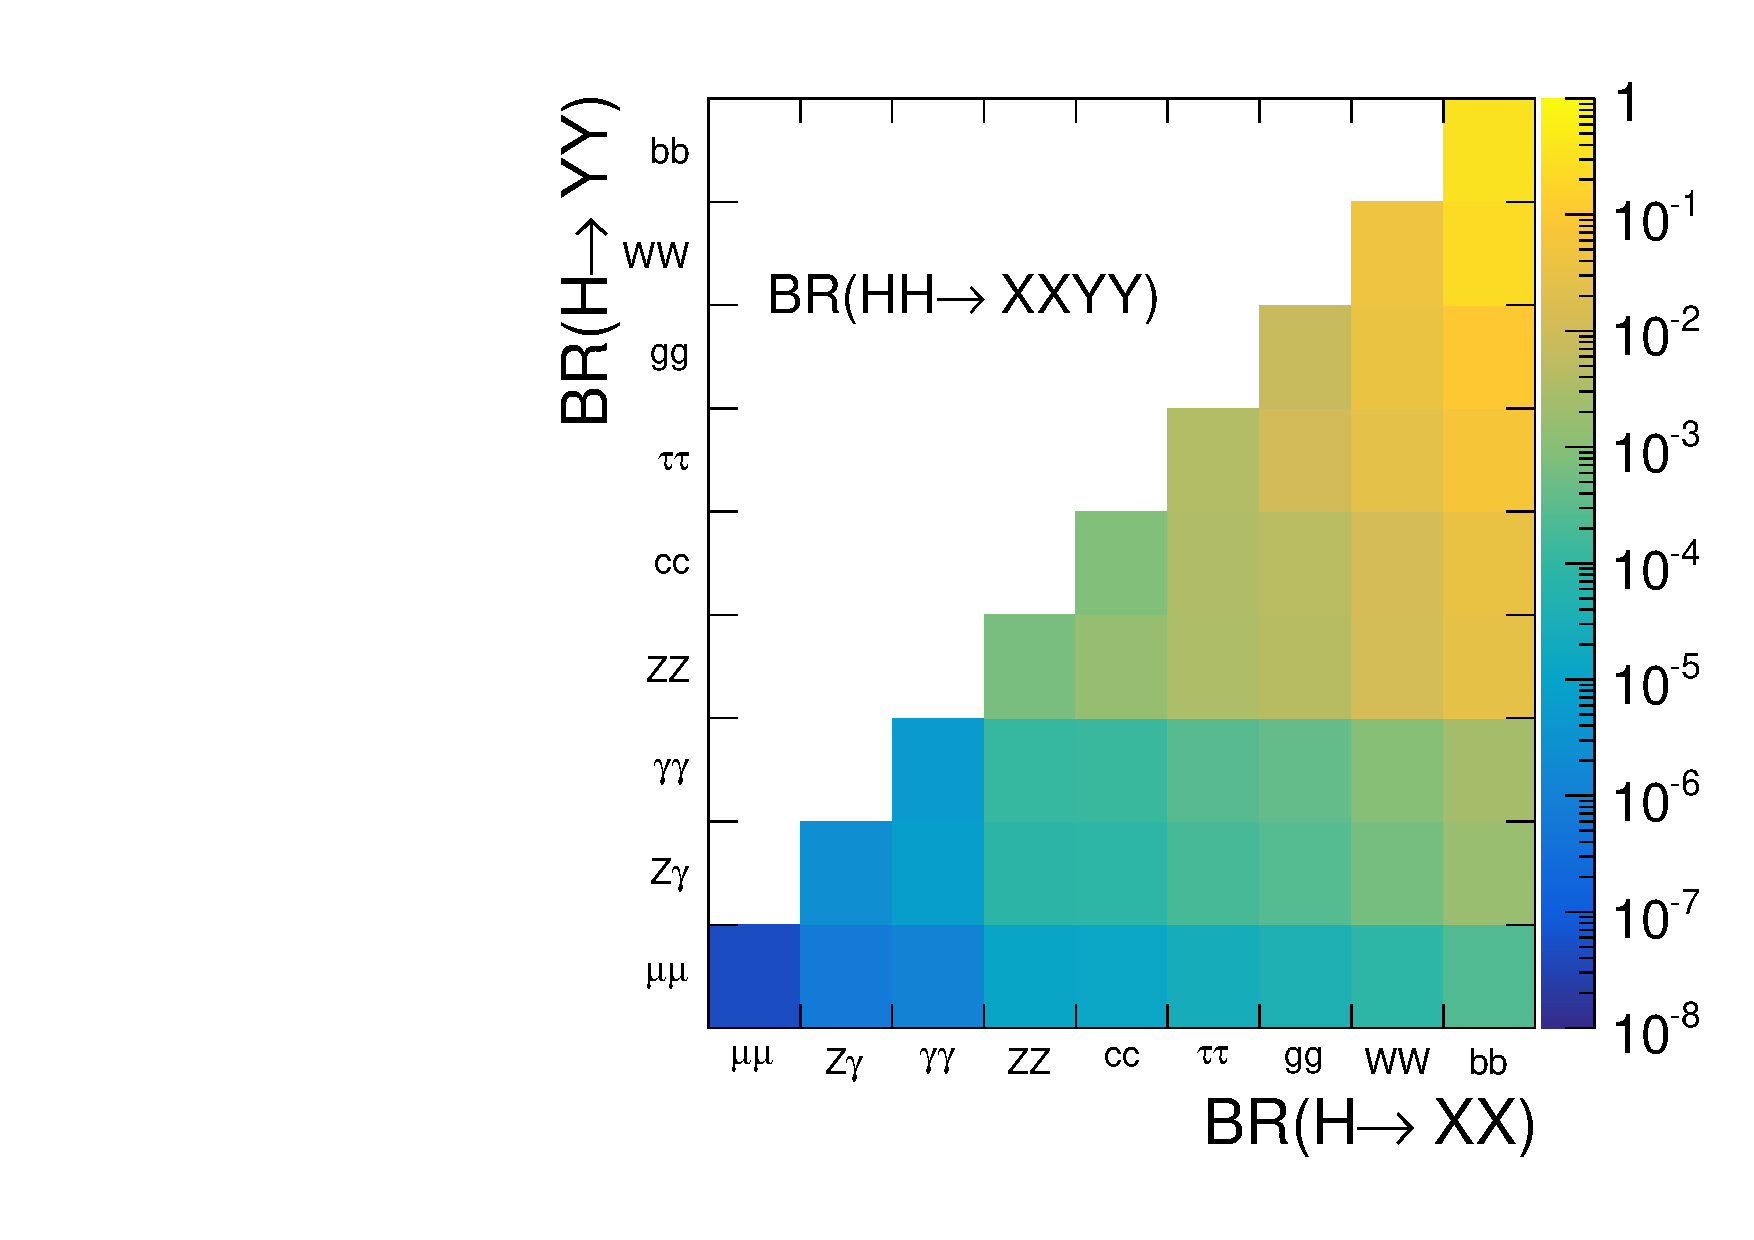
\includegraphics[width=0.50\textwidth]{BR}
    \caption[Double Higgs decay channels]{Double Higgs decay channels. The SM branching fractions are represented by the colour palette.}
    \label{BR}
\end{figure}



